A static bending test of beams in an universal testing machine (brand AROTEC)
with capacity of at least 300kN was done. The tests were conducted with samples
without defects, from  \textit{Eucalyptus Grandis}  wood, with dimensions of
$2.5 \times 2.5 \times41 cm$. The execution of the tests and the preparation 
of the samples were done based on the norm $ASTM$ $D143-94$ 
\cite{AMERICANSOCIETY}.

\subsection{System setup}
\label{subsec:syssetup}
The $PIV$ technique, in the context of parameter analyses in the static bending test of beams,
It is presented in this work as the tracking of a set of $N=3$ analysis
region (selected in an initial picture) through $M$ pictures taken in standard time intervals ($\tau$).
The Fig. \ref{fig:pivwindow} shows the first picture (left side) 
and the last picture (right side). The picture of the left was taken in
the time $t=0$ and It represents the beam in study with 
$N$ square analysis regions of $WSIZE$ pixels of side; this regions are tracked
across a set of $M$ pictures. The path is shown with red squares in the right side of
the same figure.
\begin{figure}[H]
\centering
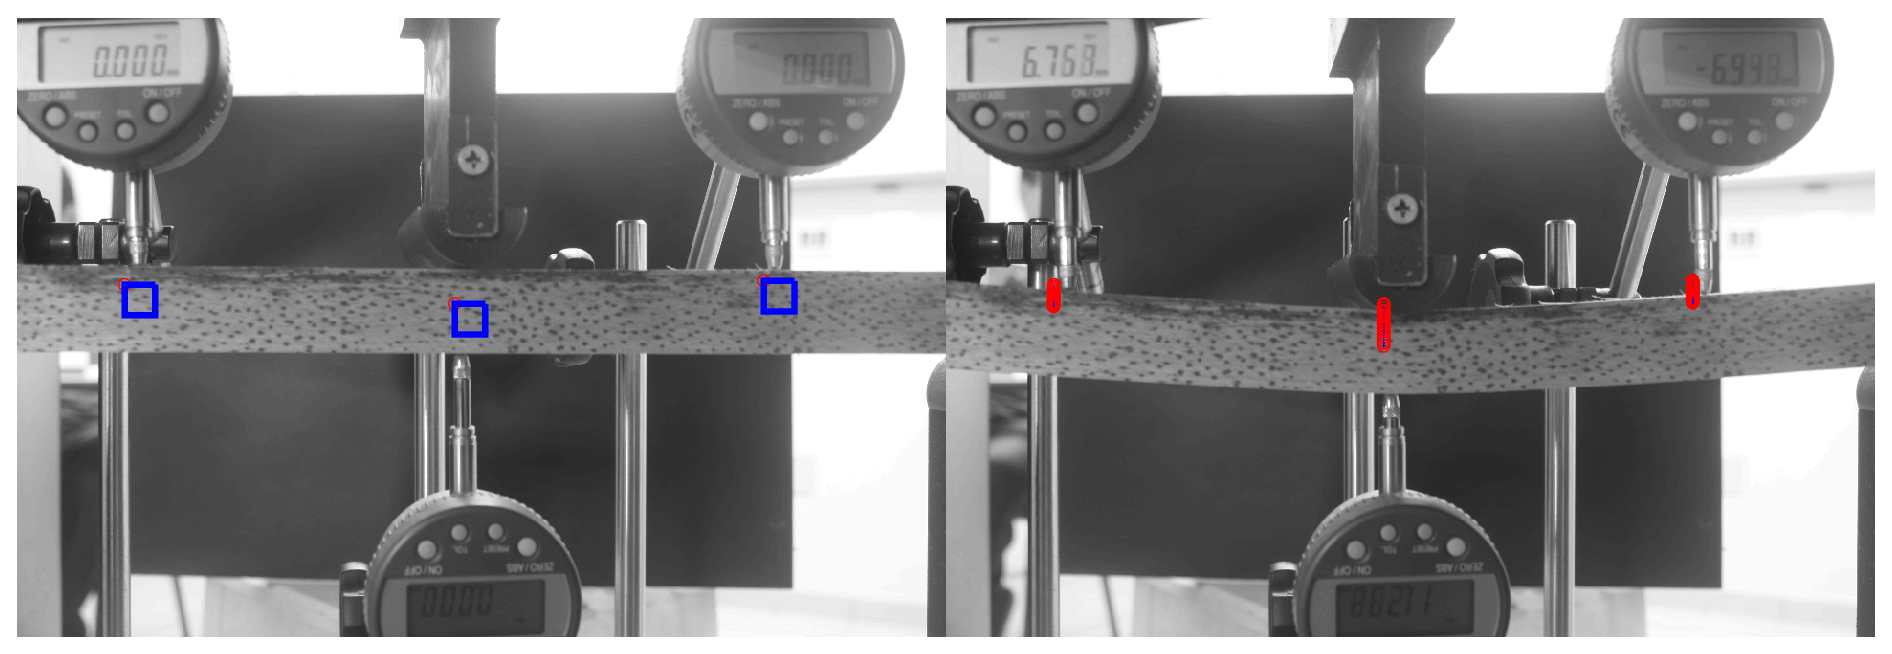
\includegraphics[width=\columnwidth]{numresult1.eps}
\caption{Followed path in a static bending test. 3 dial indicators are used,
two at the ends and one at the center of beam; additionally, in the middle we have a universal testing machine.}
\label{fig:pivwindow}
\end{figure}

Initially the static bending system was compound by a universal testing machine
and  dial indicators to measure the dislocation values of beams,
additionally a digital camera (Canon EOS Rabel T3) was positioned 
to take pictures of the tests. 
A camera was equipped with a lens set to improve
the focusing of the surface of samples; the images were taken through the use of
the remote control to minimize the external interferences in the capture time. 
The detailed arrangement of the instruments in the test can be seen in the Fig. \ref{fig:system1}.
\begin{figure}[H]
\centering
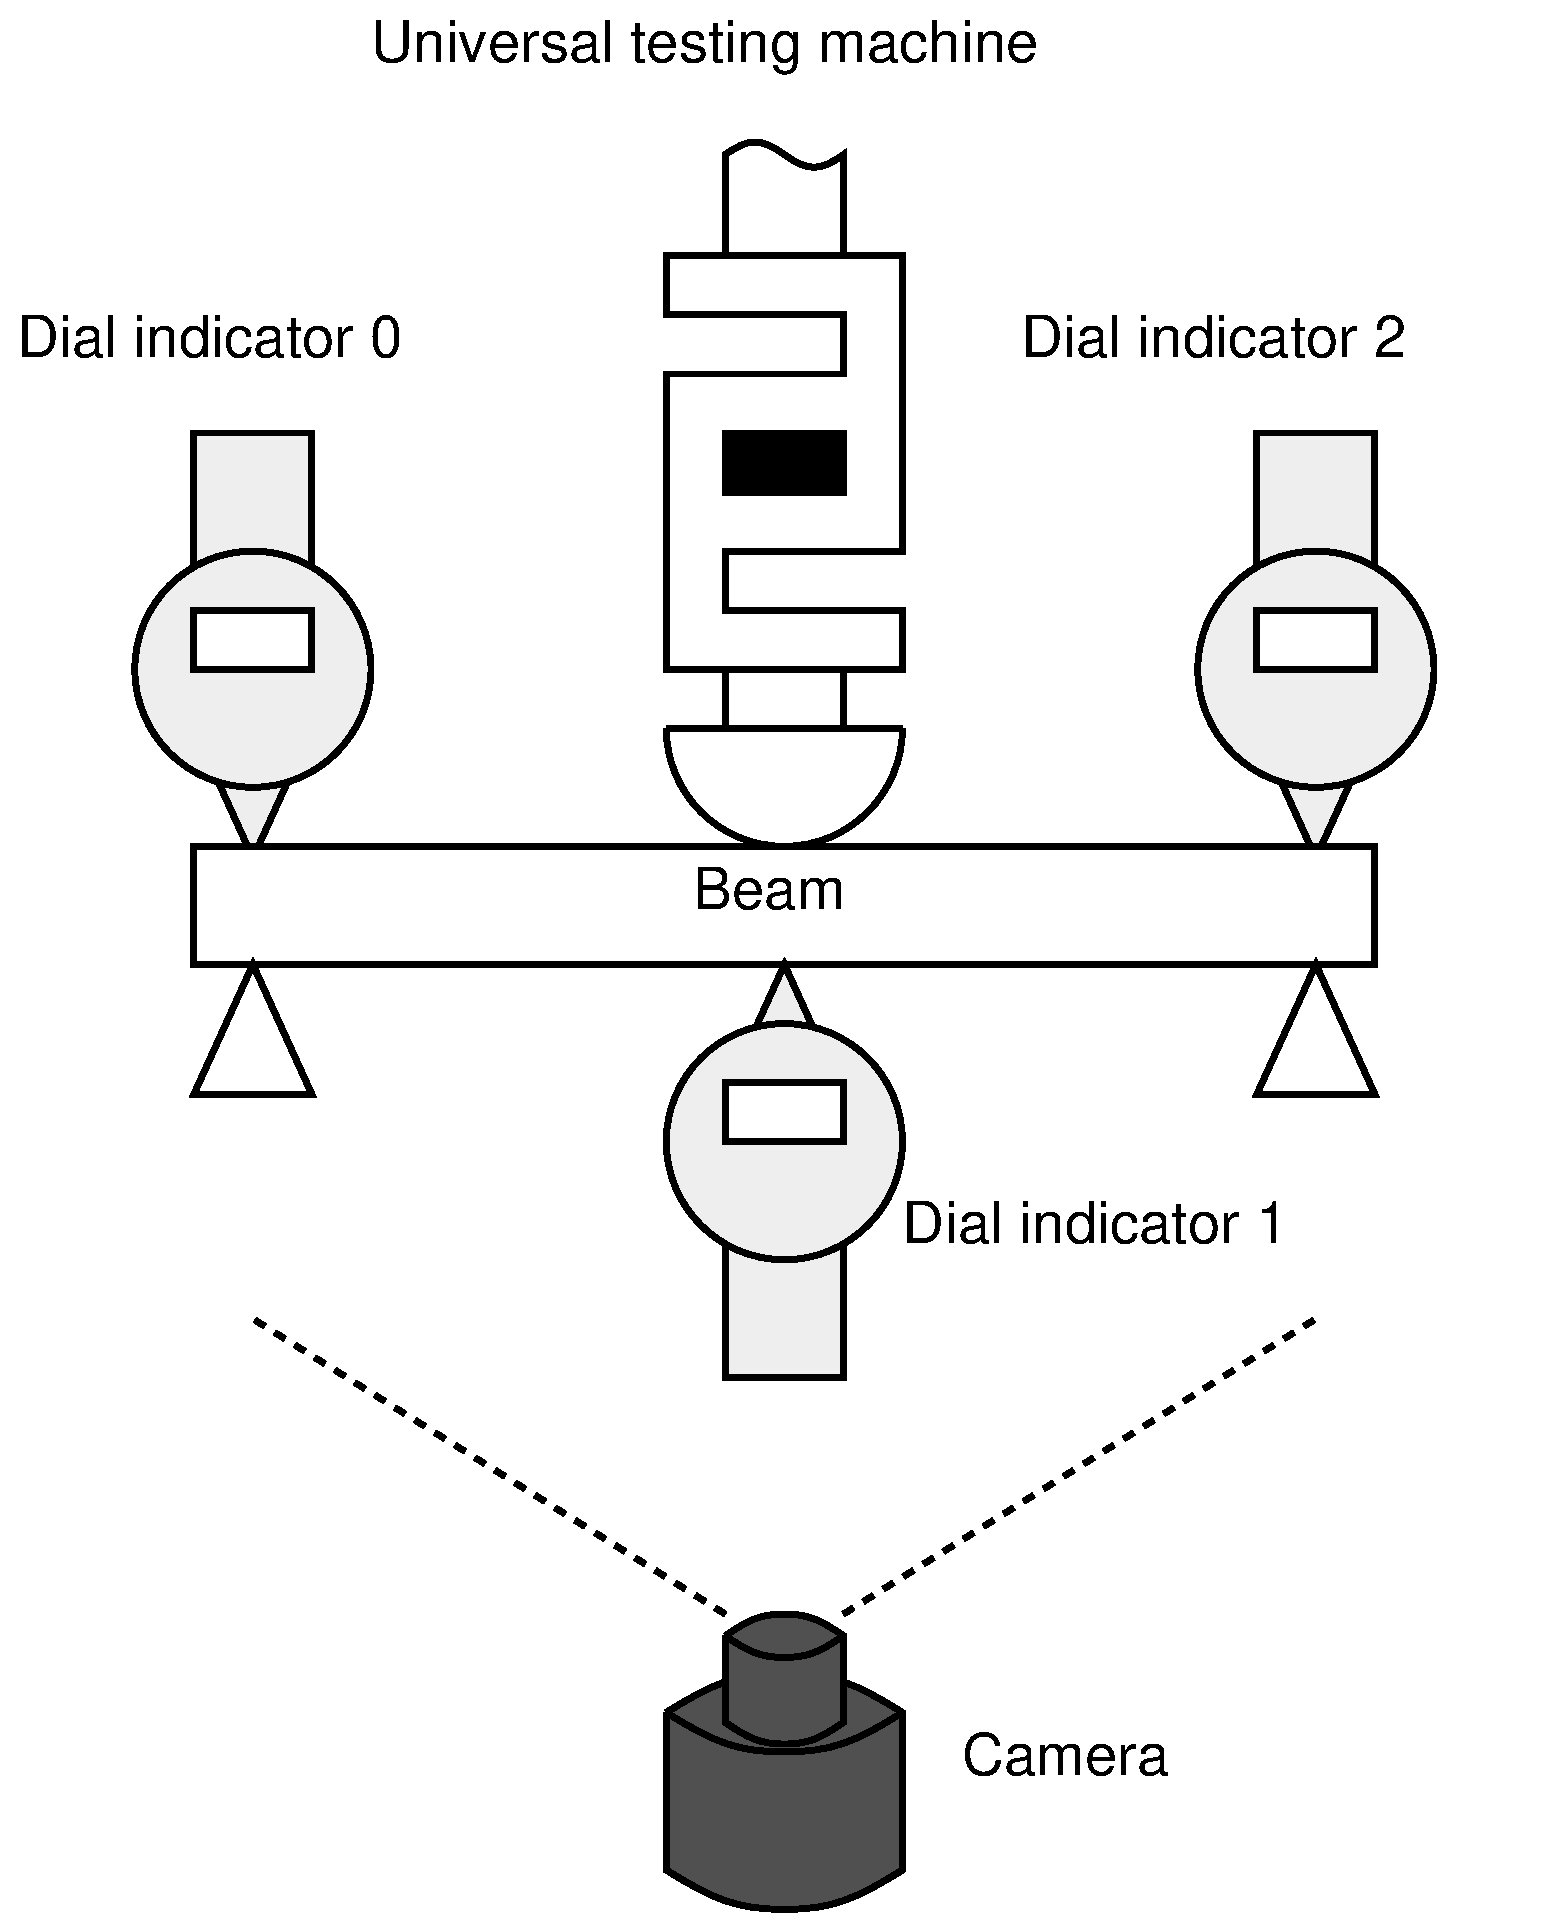
\includegraphics[width=0.45\columnwidth]{Diagrama1.eps}
\caption{System setup description.}
\label{fig:system1}
\end{figure}

In the wood samples, 3 different types of patterns were painted,
the first pattern was painted with spray ($PA$), the second was made marking points, 
with a brush pen, making a regular grid of points with 
$5$ pixels of diameter and $11$ pixels of separation ($PB$), 
and finally in the third were painted
random points of $\sim 5$ pixels of diameter and separation of $\sim 11$ 
pixels  ($PC$), see Fig. \ref{fig:samplesabc}, 
so that the $PIV$ algorithm use these points as particle groups and 
it can track them between consecutive pictures.
\begin{figure}[H]
\centering
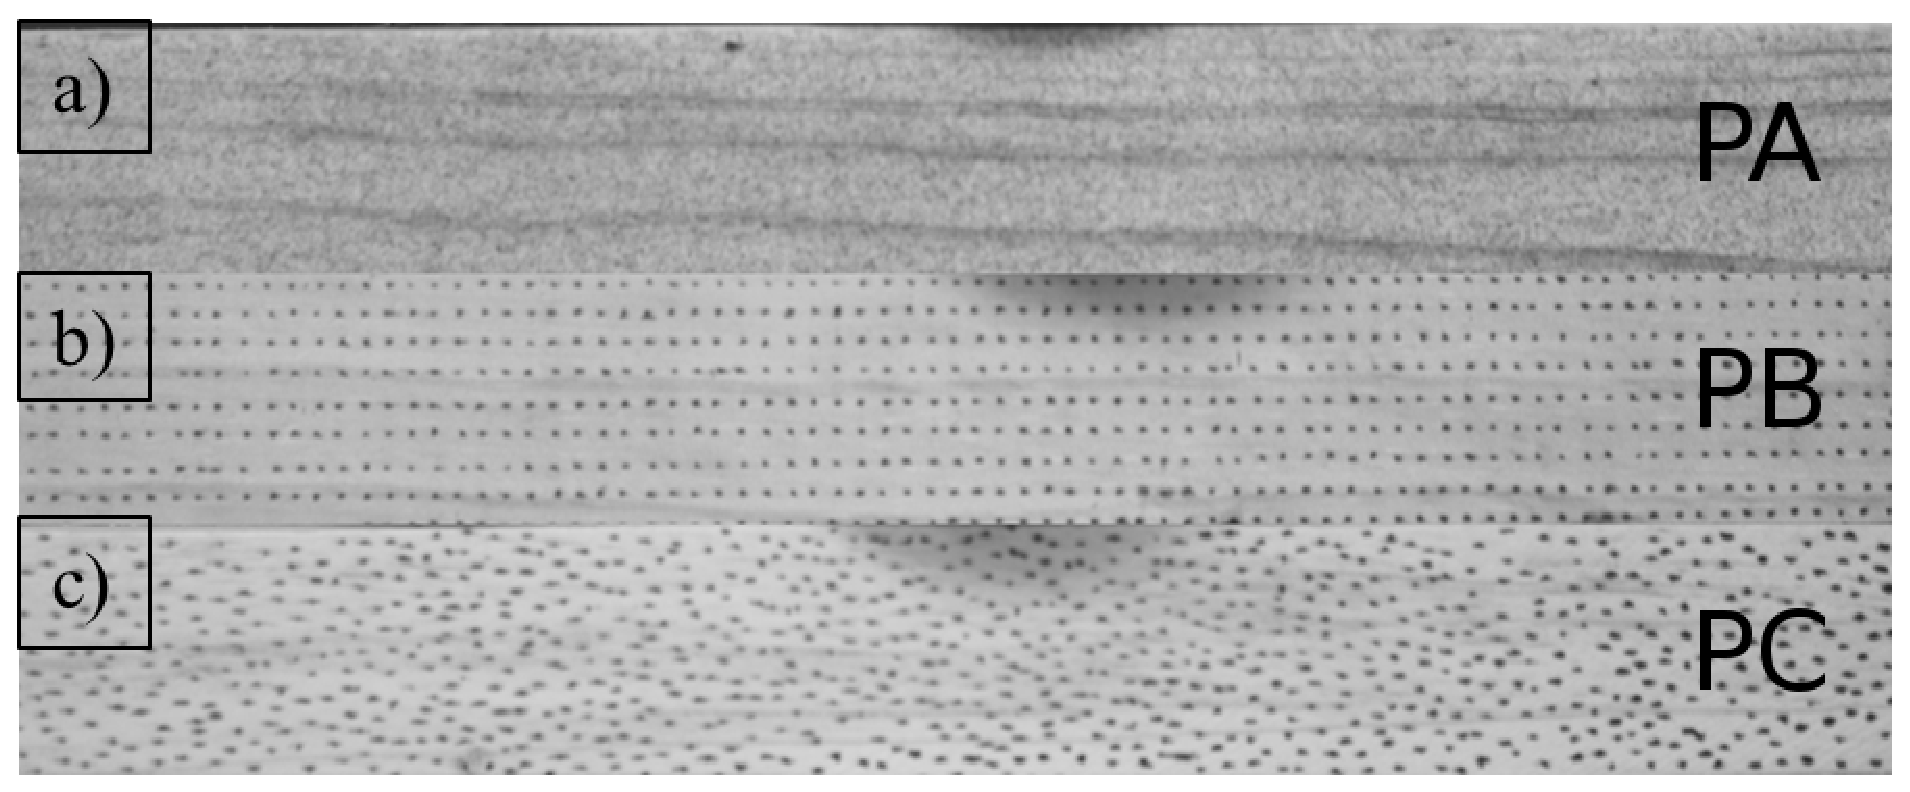
\includegraphics[width=\columnwidth]{abc.eps}
\caption{Surface of the samples with the 3 different patterns. 
$a)$ Black spray paint. $b)$ Points in regular grid with brush pen. $c)$ Random points with brush pen.}
\label{fig:samplesabc}
\end{figure}

It was pre-establishment that, the images would be taken in regular intervals of $\tau=30s$; 
this interval gave us an adequate number of images to execute the procedures. 
The first image was taken at the instant $t=0$ with displacement zero.
after the end of the test, the images were edited to decrease its size in pixels
(change the original image to 8 bit format and decreasing the number of pixels to 25\%);
this procedure is done to  achieve low computational time when
the $PIV$ algorithm is used as described in the appendix, Sec. \ref{sec:algorithm}.
